\documentclass[11pt]{article}
\usepackage{amsmath}
\usepackage{multicol}
\usepackage{booktabs}
\usepackage{color}
\usepackage{epigraph}
\usepackage{float}
\usepackage{fourier}
\usepackage{fullpage}
\usepackage{graphicx}
\usepackage{listings}
\usepackage{subcaption}
\usepackage{url}
\usepackage{wrapfig}
\usepackage{xspace}
\usepackage[colorlinks=true,urlcolor=blue]{hyperref}

\newcommand{\Bash}{\texttt{bash}\xspace}
\newcommand{\Zsh}{\texttt{zsh}\xspace}
\newcommand{\C}{\textbf{C}\xspace}
\newcommand{\Unix}{\textsc{Unix}\xspace}

\title{Assignment 1 \\ Getting Acquainted with \Unix{} and \C{}}
\author{Prof. Darrell Long \\
CSE 13S -- Winter 2022}
\date{Due: January 12$^\text{th}$ at 11:59\,pm}

\usepackage{fancyhdr}
\pagestyle{fancy}
\fancyhf{}

\fancypagestyle{plain}{%
  \fancyhf{}
  \renewcommand{\headrulewidth}{0pt}
  \renewcommand{\footrulewidth}{0pt}
  \lfoot{\textcopyright{} 2021 Darrell Long}
  \rfoot{\thepage}
}

\pagestyle{plain}

\definecolor{codegreen}{rgb}{0,0.5,0}
\definecolor{codegray}{rgb}{0.5,0.5,0.5}
\definecolor{codepurple}{rgb}{0.58,0,0.82}

\lstloadlanguages{C,make,python,fortran}

\lstdefinestyle{c99}{
    morekeywords={bool, uint8_t, uint16_t, uint32_t, uint64_t, int8_t, int16_t, int32_t, int64_t},
    commentstyle=\color{codegreen},
    keywordstyle=\color{magenta},
    numberstyle=\tiny\color{codegray},
    identifierstyle=\color{blue},
    stringstyle=\color{codepurple},
    basicstyle=\ttfamily,
    breakatwhitespace=false,
    breaklines=true,
    captionpos=b,
    keepspaces=true,
    numbers=left,
    numbersep=5pt,
    showspaces=false,
    showstringspaces=false,
    showtabs=false,
    tabsize=4
}

\newcommand{\monkey}[1]{
  \begin{center}
    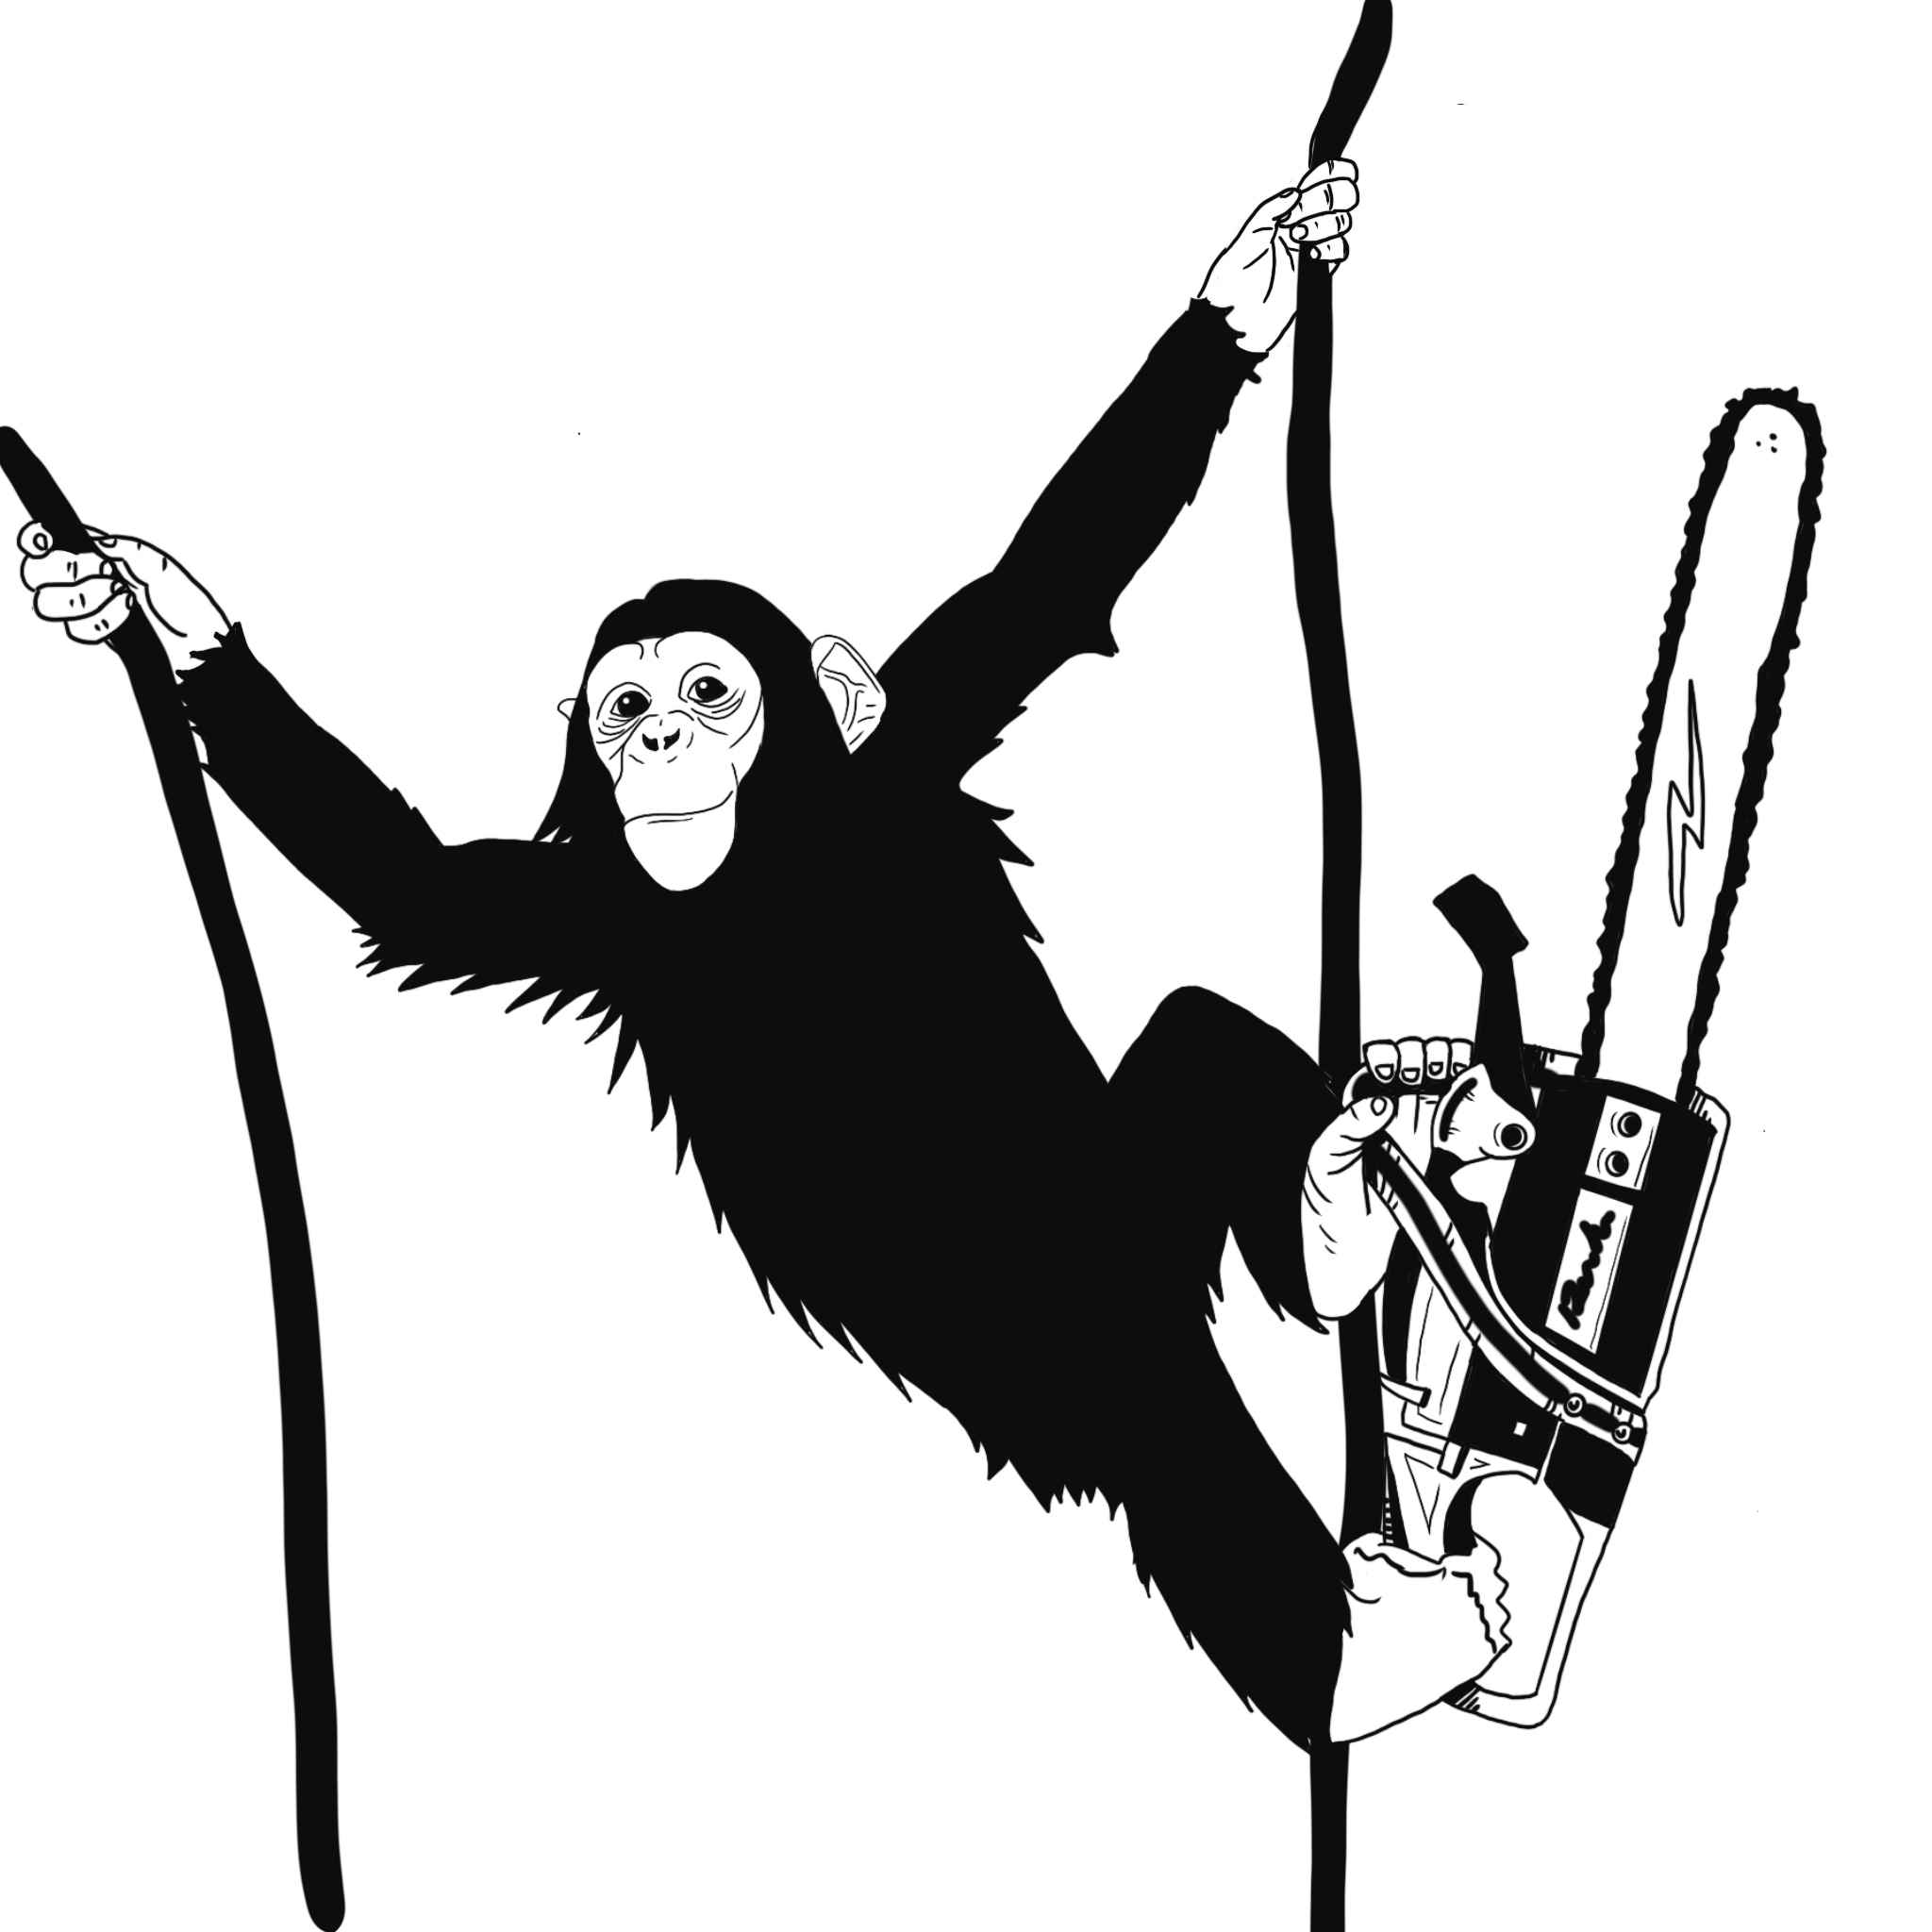
\includegraphics[width=0.35\textwidth]{../monkey.jpg} \\
    \emph{#1}
  \end{center}
}


\begin{document}\maketitle

\section{Introduction}

\epigraphwidth=0.65\textwidth
\epigraph{\emph{I wonder why it is that when I plan a route too
    carefully, it goes to pieces, whereas if I blunder along in blissful
    ignorance aimed in a fancied direction I get through with no
    trouble.}}{---John Steinbeck, \emph{Travels with Charley: In Search
    of America}}

\noindent
Denver Long decided to augment his income during his retirement
years by selling the prestigious products produced by the Shinola
Corporation.  He enjoys driving his Cadillac, so it's the life of
a traveling salesman for him.  He loads up his little dog Satan---whom
he calls \emph{Baby}---and heads out on his new career.

But his first trip does not go so well. Heading to his son's house
after visiting his new grandson, he accidentally takes a wrong turn
near Chula Vista and winds up in Mexico.  Despite many pleasant
visits to Tijuana in years past, visiting his old friend Se\~nor Vasquez
on his ranchero, shooting their rifles at an old El Dorado that he has traded to Se\~nor
Vasquez decades before,
it's no longer the familiar Mexico of 1974.  Having
no passport, and speaking very little Spanish, he turns around in
frustration.  The Border Patrol won't let him back into the United
States for many hours, until he finally wears them down through his
power of persuasion.

Since the profit of his new enterprise depends
on the cost and duration of travel, and losing a day in Tijuana
cost him a potential sale in Barstow, he asks his eldest son to
have his class create a computer program that will provide an optimal
route to all the cities along his way and then return him to his
home in scenic Clearlake.

\section{\Unix{} and the Shell}\label{section:unix}

\noindent To understand why a \emph{shell} is used to interact with
\Unix{}, we need to first delve into why \Unix{} was developed the
way it was. The development of \Unix{} started by
Ken Thompson and Dennis Ritchie, with contributions by many others, for use at Bell
Laboratories (Bell Labs). The development continued throughout most of the 70s, eventually leading
to the licensing of \Unix{} to other parties in the late 70s.

Along with \Unix{} came the \Unix{} philosophy. This philosophy is
based on the belief that a tool should have a very limited, yet specific
function. All the tools on the original \Unix{} system shipped with this
philosophy. Examples include \texttt{head}, which prints out the first $n$ lines
of a file, \texttt{ls}, which lists out files in a directory, and \texttt{diff},
which reports differences between two files. The idea is that the output of one
tool, or \emph{command}, can become the input of another command.

Commands are the main way that users are intended to interact with
\Unix{}. Each command follows the pattern of \texttt{command
[arguments]} (here the square brackets mean the arguments are
optional). Each command can be executed an optional number of
arguments. Consider the following command:

\begin{shlisting}{}
$ wc -l roster.csv
\end{shlisting}

This particular command uses the \texttt{wc} command, which is a program that
counts the number of words, lines, and characters in a file. The argument
\texttt{-l} tells \texttt{wc} to only consider the line count. The final
argument, \texttt{roster.csv}, is the file to get the line count from. Note the
\texttt{\$} prefixing the command. The \texttt{\$} it not itself part of the
command, but is commonly used to indicate that the command is run in a
\emph{shell} and acts as a \emph{shell prompt}.

A shell is a program that runs in an infinite loop, parsing and executing
commands. In other words, it acts as a \emph{command line interpreter}. Examples
of popular shells include \Bash{} and \Zsh{}. Both these shells have two modes of
operation: interactive and batch. Using a shell in interactive mode means
issuing commands one at a time, with the result of the command appearing
immediately after the command is executed. Using a shell in batch mode means
giving the shell a \emph{series} of commands to run in sequence. Typically this
means placing all the commands in a file. Files that contain a series of
commands to run are typically called \emph{shell scripts}. You will be writing a
shell script for this assignment.

\section{Gnu Plot (\texttt{gnuplot})}

\texttt{gnuplot} is a utility that can be run on a variety of platforms (Linux,
macOS, Windows, and many more) used to generate high-quality plots and graphs.
Unlike Excel, \texttt{gnuplot} is used through the command-line --- the shell.
Although you can use it interactively, issuing commands and having the current
plot be redrawn, \texttt{gnuplot} is capable of running commands in batch,
lending itself very naturally for use in a \Bash{} script. To install
\texttt{gnuplot} on Linux:

\begin{shlisting}{}
$ sudo apt install gnuplot
\end{shlisting}

\texttt{gnuplot} is mostly used to plot data points in a file. The basic format
is very simplistic: just a series of $(x, y)$ coordinates on each line, separated
by whitespace.

\begin{pylisting}{Example data file: \texttt{example.dat}.}
1 5
2 4
3 3
4 2
5 1
\end{pylisting}

After you've created this file, start up \texttt{gnuplot}. This should open up
an interactive prompt. From here, all we need to do is specify what data file to
plot and how to plot it.

\begin{shlisting}{}
$ gnuplot

        G N U P L O T
        Version 5.4 patchlevel 2    last modified 2021-06-01

        Copyright (C) 1986-1993, 1998, 2004, 2007-2021
        Thomas Williams, Colin Kelley and many others

        gnuplot home:     http://www.gnuplot.info
        faq, bugs, etc:   type "help FAQ"
        immediate help:   type "help"  (plot window: hit 'h')

Terminal type is now 'qt'
gnuplot> plot "example.dat" with linespoints
\end{shlisting}

Entering this command into \texttt{gnuplot} should result in the plot popping up
in a window. We would also like to be able to export a plot to a file, say a
PDF. We'd also prefer if we didn't have to interactively type out what to plot
each time. There is where the non-interactive mode for \texttt{gnuplot} comes
in. We can create a file listing the commands we'd ordinarily issue to
\texttt{gnuplot} interactively and instruct it to output the plot to a PDF of
our choosing.

\begin{pylisting}{Example \texttt{gnuplot} file: \texttt{example.plot}.}
set terminal pdf
set output "example.pdf"
set xlabel "x"
set ylabel "y"
plot "example.dat" with linespoints
\end{pylisting}

We now redirect the contents of \texttt{example.plot} into \texttt{gnuplot},
which should generate the plot in a file named \texttt{example.pdf}. The plot
should resemble Figure \ref{figure:example}. We'll learn more about file
redirection when we discuss basic \Bash{} scripting in \S\ref{section:bash}.

\begin{shlisting}{}
$ gnuplot < example.plot
\end{shlisting}

\begin{figure}[bth]
  \centering
  % GNUPLOT: LaTeX picture with Postscript
\begingroup
  \makeatletter
  \providecommand\color[2][]{%
    \GenericError{(gnuplot) \space\space\space\@spaces}{%
      Package color not loaded in conjunction with
      terminal option `colourtext'%
    }{See the gnuplot documentation for explanation.%
    }{Either use 'blacktext' in gnuplot or load the package
      color.sty in LaTeX.}%
    \renewcommand\color[2][]{}%
  }%
  \providecommand\includegraphics[2][]{%
    \GenericError{(gnuplot) \space\space\space\@spaces}{%
      Package graphicx or graphics not loaded%
    }{See the gnuplot documentation for explanation.%
    }{The gnuplot epslatex terminal needs graphicx.sty or graphics.sty.}%
    \renewcommand\includegraphics[2][]{}%
  }%
  \providecommand\rotatebox[2]{#2}%
  \@ifundefined{ifGPcolor}{%
    \newif\ifGPcolor
    \GPcolorfalse
  }{}%
  \@ifundefined{ifGPblacktext}{%
    \newif\ifGPblacktext
    \GPblacktexttrue
  }{}%
  % define a \g@addto@macro without @ in the name:
  \let\gplgaddtomacro\g@addto@macro
  % define empty templates for all commands taking text:
  \gdef\gplbacktext{}%
  \gdef\gplfronttext{}%
  \makeatother
  \ifGPblacktext
    % no textcolor at all
    \def\colorrgb#1{}%
    \def\colorgray#1{}%
  \else
    % gray or color?
    \ifGPcolor
      \def\colorrgb#1{\color[rgb]{#1}}%
      \def\colorgray#1{\color[gray]{#1}}%
      \expandafter\def\csname LTw\endcsname{\color{white}}%
      \expandafter\def\csname LTb\endcsname{\color{black}}%
      \expandafter\def\csname LTa\endcsname{\color{black}}%
      \expandafter\def\csname LT0\endcsname{\color[rgb]{1,0,0}}%
      \expandafter\def\csname LT1\endcsname{\color[rgb]{0,1,0}}%
      \expandafter\def\csname LT2\endcsname{\color[rgb]{0,0,1}}%
      \expandafter\def\csname LT3\endcsname{\color[rgb]{1,0,1}}%
      \expandafter\def\csname LT4\endcsname{\color[rgb]{0,1,1}}%
      \expandafter\def\csname LT5\endcsname{\color[rgb]{1,1,0}}%
      \expandafter\def\csname LT6\endcsname{\color[rgb]{0,0,0}}%
      \expandafter\def\csname LT7\endcsname{\color[rgb]{1,0.3,0}}%
      \expandafter\def\csname LT8\endcsname{\color[rgb]{0.5,0.5,0.5}}%
    \else
      % gray
      \def\colorrgb#1{\color{black}}%
      \def\colorgray#1{\color[gray]{#1}}%
      \expandafter\def\csname LTw\endcsname{\color{white}}%
      \expandafter\def\csname LTb\endcsname{\color{black}}%
      \expandafter\def\csname LTa\endcsname{\color{black}}%
      \expandafter\def\csname LT0\endcsname{\color{black}}%
      \expandafter\def\csname LT1\endcsname{\color{black}}%
      \expandafter\def\csname LT2\endcsname{\color{black}}%
      \expandafter\def\csname LT3\endcsname{\color{black}}%
      \expandafter\def\csname LT4\endcsname{\color{black}}%
      \expandafter\def\csname LT5\endcsname{\color{black}}%
      \expandafter\def\csname LT6\endcsname{\color{black}}%
      \expandafter\def\csname LT7\endcsname{\color{black}}%
      \expandafter\def\csname LT8\endcsname{\color{black}}%
    \fi
  \fi
    \setlength{\unitlength}{0.0500bp}%
    \ifx\gptboxheight\undefined%
      \newlength{\gptboxheight}%
      \newlength{\gptboxwidth}%
      \newsavebox{\gptboxtext}%
    \fi%
    \setlength{\fboxrule}{0.5pt}%
    \setlength{\fboxsep}{1pt}%
    \definecolor{tbcol}{rgb}{1,1,1}%
\begin{picture}(7200.00,5040.00)%
    \gplgaddtomacro\gplbacktext{%
      \csname LTb\endcsname%%
      \put(814,704){\makebox(0,0)[r]{\strut{}$1$}}%
      \put(814,1218){\makebox(0,0)[r]{\strut{}$1.5$}}%
      \put(814,1733){\makebox(0,0)[r]{\strut{}$2$}}%
      \put(814,2247){\makebox(0,0)[r]{\strut{}$2.5$}}%
      \put(814,2762){\makebox(0,0)[r]{\strut{}$3$}}%
      \put(814,3276){\makebox(0,0)[r]{\strut{}$3.5$}}%
      \put(814,3790){\makebox(0,0)[r]{\strut{}$4$}}%
      \put(814,4305){\makebox(0,0)[r]{\strut{}$4.5$}}%
      \put(814,4819){\makebox(0,0)[r]{\strut{}$5$}}%
      \put(946,484){\makebox(0,0){\strut{}$1$}}%
      \put(1678,484){\makebox(0,0){\strut{}$1.5$}}%
      \put(2410,484){\makebox(0,0){\strut{}$2$}}%
      \put(3142,484){\makebox(0,0){\strut{}$2.5$}}%
      \put(3875,484){\makebox(0,0){\strut{}$3$}}%
      \put(4607,484){\makebox(0,0){\strut{}$3.5$}}%
      \put(5339,484){\makebox(0,0){\strut{}$4$}}%
      \put(6071,484){\makebox(0,0){\strut{}$4.5$}}%
      \put(6803,484){\makebox(0,0){\strut{}$5$}}%
    }%
    \gplgaddtomacro\gplfronttext{%
      \csname LTb\endcsname%%
      \put(209,2761){\rotatebox{-270}{\makebox(0,0){\strut{}y}}}%
      \put(3874,154){\makebox(0,0){\strut{}x}}%
      \csname LTb\endcsname%%
      \put(5816,4646){\makebox(0,0)[r]{\strut{}"example.dat"}}%
    }%
    \gplbacktext
    \put(0,0){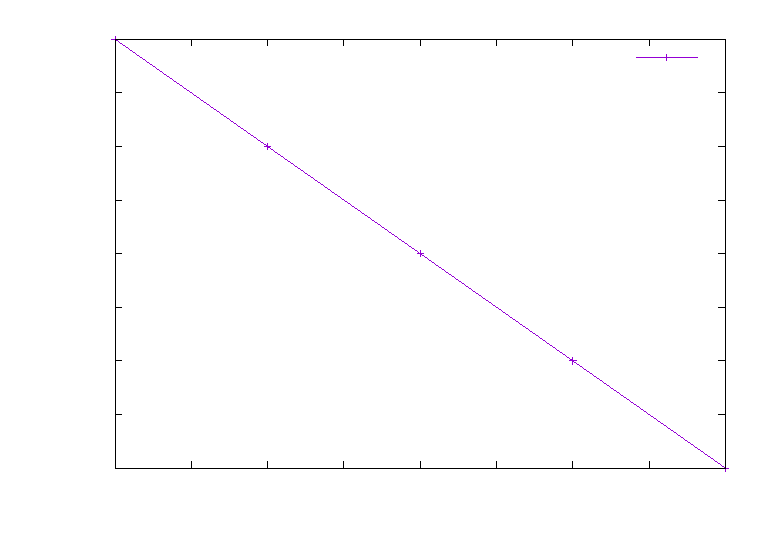
\includegraphics[width={360.00bp},height={252.00bp}]{figures/example}}%
    \gplfronttext
  \end{picture}%
\endgroup

  \caption{\label{figure:example}
    Example plot generated by \texttt{gnuplot}.
  }
\end{figure}

You can learn more about \texttt{gnuplot} and view more extensive examples,
respectively, with the following links:

\centerline{\url{http://gnuplot.info/documentation.html}}
\centerline{\url{http://gnuplot.info/demos/}}

There is also a built-in help system in \texttt{gnuplot}. Just type
``help'' when you are in interactive mode.

Do you have to use \texttt{gnuplot} for your course assignments? Yes. What about
Excel? No. What about some random online tool? No. You have to learn and use a
\Unix{} command line tool. If you are extremely insistent on not using
\texttt{gnuplot}, you can use \texttt{matplotlib} for Python as an alternative.
But you're on your own there.

\section{\LaTeX{} (\texttt{pdflatex})}

What is \LaTeX? It is a tool used by scientists, mathematicians and
engineers to produce high quality documents. It is especially
useful when your documents have mathematics in them.

Here is an example minimal \LaTeX document. There is a much more
complete example in the course resources repository. If your GitLab repository
has been created, then you should have access to this repository. It contains
the materials for each assignment: header files, source examples, and example
programs. You can access the repository here:

\vspace\baselineskip
\centerline{\url{https://git.ucsc.edu/cse13s/winter2023-section02/resources.git}}
\vspace\baselineskip

\begin{verbatim}
\documentclass[11pt]{article} % Document type
\title{Example Document}
\author{Conrad Veidt}
\date{\today} % Sets the date to \today, or any date you specify
\begin{document}\maketitle % Start the document
For the left Riemann sum, approximating the function by its value at the
left-end point gives multiple rectangles with base $\Delta x$ and height
$f(a + i\Delta x)$. Doing this for $i = 0, 1, \ldots , n-1$, and adding
up the resulting areas gives
$$
A_\text{left} =
\Delta x \left[f(a) + f(a + \Delta x)
+ f(a+ 2 \, \Delta x)+ \cdots+f(b - \Delta x)\right].
$$
\end{document}
\end{verbatim}

You will need to install \LaTeX{} before you can start using it. You will most
likely want the full installation:

\begin{shlisting}{}
$ sudo apt install texlive-full
\end{shlisting}

There is a complete example in the resources repository that you can modify.
\LaTeX{} is a compiled language, just like \C{}. That means if you make a syntax
error it will complain!

Do you have to use \LaTeX? Yes, and it works well with \texttt{gnuplot}.
Life will be much easier if you take a few minutes to learn and use
\LaTeX{}. All you need to do is to mimic what you find in the example
documents.

\section{Your Task}

\epigraphwidth=0.5\textwidth
\epigraph{\emph{The people will believe what the media tells them they
believe.}}{---George Orwell}

\noindent
\begin{itemize}
  \item Initialize your Bloom filter and hash table.
  \item Read in a list of \emph{badspeak} words with \texttt{fscanf()}.
    Again, badspeak is simply oldspeak without a newspeak translation.
    Badspeak is strictly forbidden. Each badspeak word should be added
    to the Bloom filter and the hash table. The list of proscribed words
    will be in \texttt{badspeak.txt}, which can be found in the
    \texttt{resources} repository.
  \item Read in a list of \emph{oldspeak} and \emph{newspeak} pairs with
    \texttt{fscanf()}. Only the oldspeak should be added to the Bloom
    filter. The oldspeak \emph{and} newspeak are added to the hash
    table. The list of oldspeak and newspeak pairs will be in
    \texttt{newspeak.txt}, which can also be found in the
    \texttt{resources} repository.
  \item Now that the lexicon of badspeak and oldspeak/newspeak
    translations has been populated, you can start to filter out words.
    Read words in from \texttt{stdin} using the supplied parsing module.
  \item For each word that is read in, check to see if it has been added
    to the Bloom filter. If it has not been added to the Bloom filter,
    then no action is needed since the word isn't a proscribed word.
  \item If the word has most likely been added to the Bloom filter,
    meaning \texttt{bf\_probe()} returned \texttt{true}, then further
    action needs to be taken.
    \begin{enumerate}
      \item If the hash table contains the word and the word \emph{does
        not} have a newspeak translation, then the citizen who used this
        word is guilty of \texttt{thoughtcrime}. Insert this badspeak
        word into a list of badspeak words that the citizen used in
        order to notify them of their errors later. What data structure
        could be used to store these words?
      \item If the hash table contains the word, and the word \emph{does}
        have a newspeak translation, then the citizen requires
        counseling on proper \emph{Rightspeak}. Insert this oldspeak
        word into a list of oldspeak words with newspeak translations in
        order to notify the citizen of the revisions needed to be made
        in order to practice Rightspeak.
      \item If the hash table does not contain the word, then all is
        good since the Bloom filter issued a false positive. No
        disciplinary action needs to be taken.
    \end{enumerate}
  \item If the citizen is accused of thoughtcrime \emph{and} requires
    counseling on proper \emph{Rightspeak}, then they are given a
    reprimanding \emph{mixspeak message} notifying them of their
    transgressions and promptly sent off to \emph{joycamp}. The message
    should contain the list of badspeak words that were used followed by
    the list of oldspeak words that were used with their proper newspeak
    translations.

  \begin{shlisting}{}
Dear beloved citizen of the GPRSC,

We have some good news, and we have some bad news.
The good news is that there is bad news. The bad news is that you will
be sent to joycamp and subjected to a week-long destitute existence.
This is the penalty for using degenerate words, as well as using
oldspeak in place of newspeak. We hope you can correct your behavior.

Your transgressions, followed by the words you must think on:

kalamazoo
antidisestablishmentarianism
write -> papertalk
sad -> happy
read -> papertalk
music -> noise
liberty -> badfree\end{shlisting}

  \item If the citizen is accused solely of thoughtcrime, then they are
    issued a thoughtcrime message and also sent off to \emph{joycamp}.
    The \emph{badspeak message} should contain the list of badspeak
    words that were used.

  \begin{shlisting}{}
Dear beloved citizen of the GPRSC,

You have been caught using degenerate words that may cause
distress among the moral and upstanding citizens of the GPSRC.
As such, you will be sent to joycamp. It is there where you will
sit and reflect on the consequences of your choice in language.

Your transgressions:

kalamazoo
antidisestablishmentarianism\end{shlisting}

  \item If the citizen only requires counseling, then they are issued an
    encouraging \emph{goodspeak message}. They will read it, correct
    their \emph{wrongthink}, and enjoy the rest of their stay in the
    GPRSC. The message should contain the list of oldspeak words that
    were used with their proper newspeak translations.

    \begin{shlisting}{}
Dear beloved citizen of the GPRSC,

We recognize your efforts in conforming to the language standards
of the GPSRC. Alas, you have been caught uttering questionable words
and thinking unpleasant thoughts. You must correct your wrongspeak
and badthink at once. Failure to do so will result in your deliverance
to joycamp.

Words that you must think on:

write -> papertalk
sad -> happy
read -> papertalk
music -> noise
liberty -> badfree\end{shlisting}

  \item Each of the messages are defined for you in \texttt{messages.h}.
    \textcolor{red}{You may not modify this file}.

  \item The list of the command-line options your program must support
    is listed below. \emph{Any} combination of the command-line options
    must be supported.
    \begin{itemize}
      \item \texttt{-h} prints out the program usage. Refer to the
      reference program in the resources repository for what to print.
      \item \texttt{-t size} specifies that the hash table
        will have \texttt{size} entries (the default will be $2^{16}$).
      \item \texttt{-f size} specifies that the Bloom filter
        will have \texttt{size} entries (the default will be $2^{20}$).
      \item \texttt{-s} will enable the printing of statistics to
        \texttt{stdout}. The statistics to calculate are:
        \begin{itemize}
          \item Average binary search tree size
          \item Average binary search tree height
          \item Average branches traversed
          \item Hash table load
          \item Bloom filter load
        \end{itemize}
        The latter three statistics are computed as follows:
        \begin{align*}
          \text{Average branches traversed} &=
          \frac{\texttt{branches}}{\texttt{lookups}} \\
          \text{Hash table load} &= 100 \times \frac{\texttt{ht\_count()}}{\texttt{ht\_size()}} \\
          \text{Bloom filter load} &= 100 \times \frac{\texttt{bf\_count()}}{\texttt{bf\_size()}}
        \end{align*}
        The hash table load and Bloom filter load should be printed with
        up to 6 digits of precision. \textcolor{red}{Enabling the
        printing of statistics should \emph{suppress all messages} the
        program may otherwise print.} The number of lookups is defined
        as the number of times \texttt{ht\_lookup()} and
        \texttt{ht\_insert()} is called. The number of branches is
        defined as the count of links traversed during calls to
        \texttt{bst\_find()} and \texttt{bst\_insert()}. The global
        variable \texttt{lookups} should be defined in \texttt{ht.c} and
        the global variable \texttt{branches} should be defined in
        \texttt{bst.c}.
    \end{itemize}
\end{itemize}

\section{\Bash{}}\label{section:bash}

We will preface this section by saying this is by no means the most
comprehensive guide to scripting in \Bash{}. For such a guide, a copy of the official \Bash{} guide can be found here:

\vspace\baselineskip
\centerline{\url{https://folk.ntnu.no/geirha/bashguide.pdf}}
\vspace\baselineskip

The amount of \Bash{} knowledge needed for this assignment is very minimal, but
will be crucial to your career in Computer Science. We will start with issuing
commands in \Bash{}. \begin{bfseries}
  \color{red} You will want to study this section and reference it in the future.
\end{bfseries}

\subsection{Commands and Arguments}

Commands in \Bash{} are made of up words delimited by whitespace, where a word is
just a sequence of characters. Most commands usually span a single line, but it
is possible to write a more complex command that spans across several lines. As
stated in \S\ref{section:unix}, a command follows the pattern \texttt{command
[arguments]}. Consider the following command:

\begin{shlisting}{}
$ head notes.txt
\end{shlisting}

\Bash{} parses this specific command into two words: \texttt{head} and
\texttt{notes.txt}. The command to execute is \texttt{head} and its sole
argument is \texttt{notes.txt}. The program \texttt{head}, by default, prints
out the first $10$ lines of a specified file, in this case \texttt{notes.txt},
to \emph{standard output}, or \texttt{stdout}. This is what you think of as the
console, or terminal window. Any \Unix{} process has the following three open
input/output streams open at creation:

\begin{enumerate}
  \item Standard input (\texttt{stdin}) -- Unix file descriptor number 0
  \item Standard output (\texttt{stdout}) -- Unix file descriptor number 1
  \item Standard error (\texttt{stderr}) -- Unix file descriptor number 2
\end{enumerate}

What is a \Unix{} process? We'll learn more about that later on in the course,
but for now you can think of it as a program in execution. We'll also discuss
input and output more in-depth later on in this section. Returning back to the
discussion about arguments, it's important to note that there can be any number
of arguments to a command. For instance, the \texttt{head} program also accepts
arguments to specify how many lines of a file to print out. For example, to
print out the first 2 lines of \texttt{notes.txt}:

\begin{shlisting}{}
$ head -n 2 notes.txt
\end{shlisting}

There's not a whole lot more to discuss regarding commands and arguments other
than the different kinds of commands: aliases, functions, built-ins, keywords,
and executables. We will only concern ourselves with built-ins and executables
for now, as they are the bare minimum needed to get moving around in \Unix{} and
writing \Bash{} scripts.

\subsection{Built-ins}

\emph{Built-ins} are functions that are built into \Bash{}. A \Bash{} function
can accept arguments and is composed of a series of commands to execute. For
example, here is a function called \texttt{mkcd} that creates a directory and
enters the created directory:

\begin{shlisting}{}
$ function mkcd { mkdir $1 && cd $1 }
\end{shlisting}

Let's break down this function a bit more. \texttt{mkdir} is a utility that
creates a directory. A directory is the equivalent of a Windows folder. The
\texttt{\$1} accesses the first argument passed to the function. This operates
by parameter expansion (more on this later), as commented in the following
example:

\begin{shlisting}{}
$ mkcd directory # Runs "mkdir directory && cd directory".
\end{shlisting}

The \texttt{\&\&} is a \emph{control operator} and indicates logical AND. So
basically, make the directory with \texttt{mkdir} \emph{and} enter it with
\texttt{cd}. \texttt{cd} is arguably one of the most important built-ins since
its sole purpose is to move around directories. \texttt{echo} is another
built-in.

\subsection{Executables}

An executable on \Unix{} is just another name for a program. The terms
\emph{program}, \emph{executable}, \emph{executable binary}, and sometimes just
\emph{binary}, all refer to a program that can be run, or \emph{executed}. The
distinction between an plain old executable and an executable binary is in its
representation. An executable binary is platform specific and is simply a file
full of machine code: pure binary. An executable could be a shell script, which
contains readable text. The only thing these two share is that they must have
the executable bit set in order to be run. Refer to the discussion of \Unix{}
file permissions in assignment 0 if you have forgotten what the executable bit
refers to.

\subsection{Parameters}

Parameters in \Bash{} store values. There are two kinds of parameters:
\emph{variables} and \emph{special parameters}. Variables are used to store
values specified by the programmer. Special parameters have values that are set
by \Bash{} itself. The value of a parameter can be accessed via \emph{parameter
expansion}, which just means prefixing a parameter's name with a \texttt{\$}. A
parameter name can consist of letters, numbers, and underscores, but cannot
start with a number. An example of \Bash{} variable assignment and parameter
expansion:

\begin{shlisting}{}
$ greeting="Bonjour"
$ prime=13
$ echo $greeting # Prints "Bonjour".
\end{shlisting}

Note that \Bash{} \emph{does not} allow spaces around the assignment operator
due how words are delimited by whitespace. Adding spaces would cause the
assignment to be parsed as three different words instead of one. Special
parameters include \texttt{@} and \texttt{?}, and even \texttt{1} that was used
in an earlier example. Each of these can also be expanded. \texttt{\$@} expands
to all the arguments passed to a command. \texttt{\$?} expands to the exit status
of the last run command. This is typically $0$ for a successful exit, and
non-zero for an unsuccessful exit. \texttt{\$1} expands to the first argument
supplied to a command.

\subsection{Conditionals}

Conditionals allow programming languages to handle decisions and take form as
expressions that can be evaluated as either true or false. \Bash{} uses a
command called \texttt{test} to test whether or not an expression is true. If an
expression is true, \texttt{test} exits with an exit code of 0. Otherwise, it
exits with an exit code of 1. For example:

\begin{shlisting}{}
$ test "hello = hello"
$ echo $? # Prints out last command's exit code, which is 0.
$ test "hello = goodbye"
$ echo $? # Prints 1.
\end{shlisting}

\Bash{}, unlike several programming languages, uses \texttt{=} instead of
\texttt{==} to test for equality. As you may expect, \Bash{} also provides
\texttt{if-else} statements.

\begin{shlisting}{}
$ if [ -f mystery ]; then echo "file"; else echo "directory"; fi
\end{shlisting}

This example tests if \texttt{mystery} is a file. The square brackets indicate a
test (\texttt{[} is a reserved keyword for the \texttt{test} command), and
\texttt{-f} tests if its argument is a file. \Bash{} has a more robust keyword
for testing, \texttt{[[}, which should be preferred over \texttt{[} since it
provides more functionality.

\begin{shlisting}{}
$ if [[ -d mystery ]]; then echo "directory"; else echo "file"; fi
\end{shlisting}

\subsection{Loops}

Loops allow for commands to be executed multiple times in succession. We will
discuss the \texttt{while} and \texttt{for}-loop in \Bash{}, since they also
appear in \textbf{C}. The \texttt{while}-loop loops until a command exits
unsuccessfully.

\begin{shlisting}{}
$ while true; do echo "infinitely looping"; done
\end{shlisting}

There are two \texttt{for}-loop flavors. One of them closely resembles a
\texttt{for}-loop in \C{}.

\begin{shlisting}{}
$ for (( i=0; i < 10; i++ )); do echo $i; done
\end{shlisting}

What is the \texttt{(( ... ))}? That is an \emph{arithmetic context} in \Bash{}.
\Bash{} inherently handles variables as just text. Try the following example:

\begin{shlisting}{}
$ x=3
$ y=29
$ if [[ $x > $y ]]; then echo "x > y"; else echo "x <= y"; fi
\end{shlisting}

Why does it print \texttt{"x > y"}? Because it compared \texttt{x} and
\texttt{y} \emph{lexicographically}. To test things numerically, we need to use
an arithmetic context.

\begin{shlisting}{}
$ x=3
$ y=29
$ if (( $x > $y )); then echo "x > y"; else echo "x <= y"; fi
\end{shlisting}

You can think of an arithmetic context as just an environment in which numerical
operations such as addition and multiplication can be performed. This is needed
for the \texttt{for}-loop because \texttt{++} is the \emph{postfix increment
operator}. You will learn more about the differences between the postfix and
prefix operators when you start writing \C{} programs.

The other \texttt{for}-loop in \Bash{} uses \emph{brace expansion}, like so:

\begin{shlisting}{}
$ for i in {0..9}; do echo $i; done
\end{shlisting}

\Bash{} handles \texttt{\{0..9\}} by expanding it to the list of words \texttt{0
1 2 3 4 5 6 7 8 9}. The variable \texttt{i} is then assigned to each expanded
word in sequence. The \texttt{..} indicates a \emph{range} in \Bash{}. Ranges in
\Bash{} are inclusive.

You can iterate over more than just integers in \Bash{}; you can even iterate
over all the files in the current directory that end in \texttt{.txt}.

\begin{shlisting}{}
$ for f in *.txt; do echo "$f seems like a text file"; done
\end{shlisting}

The \texttt{*} used in the \texttt{for}-loop is a \emph{glob}. Globs are used
for matching patterns. The \texttt{*} glob in particular matches any string.
Thus, \texttt{*.txt} matches any string as long as it ends with \texttt{.txt}.
Globs are very closely related to \emph{regular expressions}, which you'll
become acquainted with later on in the course.

\subsection{Input and Output}

As stated earlier, any \Unix{} process starts up with \texttt{stdin},
\texttt{stdout}, and \texttt{stderr}. We described them as input/output streams
earlier, but that was a slight lie. To be more exact, these are all \emph{file
descriptors}. File descriptors are simply integers that act as indices into a
table of open files for a process. By default, \texttt{stdin} is file descriptor
number 0, \texttt{stdout} is file descriptor number 1, and \texttt{stderr} is file descriptor
number 2. \texttt{stdin} is where input goes, such as a typed password when a program
prompts for one. \texttt{stdout} and \texttt{stderr} both print to the console,
with the only difference being that \texttt{stderr} is usually designated for
error messages. \Bash{} has two main mechanisms to provide input/output
redirection: \emph{file redirection}, and \emph{pipes}.

\subsubsection{File Redirection}

File redirection works for both input and output. That is, you can specify that
a program take input from a file (redirecting \texttt{stdin}) and place its
output into another file (redirecting \texttt{stdout}).

\begin{shlisting}{}
$ head < full.txt > first10.txt
\end{shlisting}

This example first redirects the \texttt{stdin} of \texttt{head} to
\texttt{full.txt}. In other words, it feeds the contents of \texttt{full.txt} to
\texttt{head}. Then, the \texttt{stdout} of \texttt{head} is redirected to
\texttt{first10.txt}. This takes the output produced by \texttt{head} and places
it in \texttt{first10.txt}. As you can imagine, \texttt{<} is the input
redirection keyword and \texttt{>} is the output redirection keyword. To
redirect \texttt{stderr}, prefix the output redirect keyword with the file
descriptor of \texttt{stderr}: $2$.

\begin{shlisting}{}
$ head < full.txt > first10.txt 2> errors.txt
\end{shlisting}

We can build on this example further, redirecting \texttt{stdout} to
\texttt{/dev/null}, then redirecting \texttt{stderr} to what \texttt{stdout} is
pointing at. \texttt{/dev/null} can be thought of as a black hole: it consumes
anything that is written to it. Note that \texttt{>} by default redirects
\texttt{stdout}. We could also manually specify to redirect \texttt{stdout} with
\texttt{1>}.

\begin{shlisting}{}
$ head < full.txt > /dev/null 2>&1
\end{shlisting}

\subsubsection{Pipes}

It is with \emph{pipes} where you can truly see and appreciate the beauty of the
\Unix{} philosophy. Pipes, originally called \emph{hoses}, allow for the
\texttt{stdout} of one process to be connected, or piped, to the \texttt{stdin}
of another process.

\begin{shlisting}{}
$ ls | sort -r
\end{shlisting}

This is an example of a \Unix{} \emph{pipeline}: two or more commands piped
together. This particular pipeline lists the contents of the current directory
in reverse lexicographic order. Hopefully it's easy to see why the \Unix{}
philosophy is so loved and still widely used today. Just consider the following
example, which prints out your most commonly used commands and the number of
times you've used the command.

\begin{shlisting}{}
$ history | awk '{ $1=""; print $0 }' | sort | uniq -c | sort -nr
\end{shlisting}

\subsection{Here-Documents}

A \emph{here-document}, or \emph{heredoc}, is another way of passing data into a
command. This is typically used if you don't have too much information to pass
along to a command and don't want to write it to a file first and then redirect
it. We'll use an example of a here-document in the next section when we tackle a
simple script using \texttt{gnuplot}.

\subsection{A Simple \Bash{} Script}

We can now start to write \Bash{} scripts. We'll start with a simple script that
plots the function $\sin(x)$ using values of $x$ within the range $[-2\pi,
2\pi)$ in increments of 0.01. This script is provided as \texttt{plot.sh} in
resource repository. Refer to Figure \ref{figure:sinplot} for what the
produced plot should resemble.

\begin{figure}[htb]
  \centering
  % GNUPLOT: LaTeX picture with Postscript
\begingroup
  \makeatletter
  \providecommand\color[2][]{%
    \GenericError{(gnuplot) \space\space\space\@spaces}{%
      Package color not loaded in conjunction with
      terminal option `colourtext'%
    }{See the gnuplot documentation for explanation.%
    }{Either use 'blacktext' in gnuplot or load the package
      color.sty in LaTeX.}%
    \renewcommand\color[2][]{}%
  }%
  \providecommand\includegraphics[2][]{%
    \GenericError{(gnuplot) \space\space\space\@spaces}{%
      Package graphicx or graphics not loaded%
    }{See the gnuplot documentation for explanation.%
    }{The gnuplot epslatex terminal needs graphicx.sty or graphics.sty.}%
    \renewcommand\includegraphics[2][]{}%
  }%
  \providecommand\rotatebox[2]{#2}%
  \@ifundefined{ifGPcolor}{%
    \newif\ifGPcolor
    \GPcolorfalse
  }{}%
  \@ifundefined{ifGPblacktext}{%
    \newif\ifGPblacktext
    \GPblacktexttrue
  }{}%
  % define a \g@addto@macro without @ in the name:
  \let\gplgaddtomacro\g@addto@macro
  % define empty templates for all commands taking text:
  \gdef\gplbacktext{}%
  \gdef\gplfronttext{}%
  \makeatother
  \ifGPblacktext
    % no textcolor at all
    \def\colorrgb#1{}%
    \def\colorgray#1{}%
  \else
    % gray or color?
    \ifGPcolor
      \def\colorrgb#1{\color[rgb]{#1}}%
      \def\colorgray#1{\color[gray]{#1}}%
      \expandafter\def\csname LTw\endcsname{\color{white}}%
      \expandafter\def\csname LTb\endcsname{\color{black}}%
      \expandafter\def\csname LTa\endcsname{\color{black}}%
      \expandafter\def\csname LT0\endcsname{\color[rgb]{1,0,0}}%
      \expandafter\def\csname LT1\endcsname{\color[rgb]{0,1,0}}%
      \expandafter\def\csname LT2\endcsname{\color[rgb]{0,0,1}}%
      \expandafter\def\csname LT3\endcsname{\color[rgb]{1,0,1}}%
      \expandafter\def\csname LT4\endcsname{\color[rgb]{0,1,1}}%
      \expandafter\def\csname LT5\endcsname{\color[rgb]{1,1,0}}%
      \expandafter\def\csname LT6\endcsname{\color[rgb]{0,0,0}}%
      \expandafter\def\csname LT7\endcsname{\color[rgb]{1,0.3,0}}%
      \expandafter\def\csname LT8\endcsname{\color[rgb]{0.5,0.5,0.5}}%
    \else
      % gray
      \def\colorrgb#1{\color{black}}%
      \def\colorgray#1{\color[gray]{#1}}%
      \expandafter\def\csname LTw\endcsname{\color{white}}%
      \expandafter\def\csname LTb\endcsname{\color{black}}%
      \expandafter\def\csname LTa\endcsname{\color{black}}%
      \expandafter\def\csname LT0\endcsname{\color{black}}%
      \expandafter\def\csname LT1\endcsname{\color{black}}%
      \expandafter\def\csname LT2\endcsname{\color{black}}%
      \expandafter\def\csname LT3\endcsname{\color{black}}%
      \expandafter\def\csname LT4\endcsname{\color{black}}%
      \expandafter\def\csname LT5\endcsname{\color{black}}%
      \expandafter\def\csname LT6\endcsname{\color{black}}%
      \expandafter\def\csname LT7\endcsname{\color{black}}%
      \expandafter\def\csname LT8\endcsname{\color{black}}%
    \fi
  \fi
    \setlength{\unitlength}{0.0500bp}%
    \ifx\gptboxheight\undefined%
      \newlength{\gptboxheight}%
      \newlength{\gptboxwidth}%
      \newsavebox{\gptboxtext}%
    \fi%
    \setlength{\fboxrule}{0.5pt}%
    \setlength{\fboxsep}{1pt}%
    \definecolor{tbcol}{rgb}{1,1,1}%
\begin{picture}(7200.00,5040.00)%
    \gplgaddtomacro\gplbacktext{%
      \csname LTb\endcsname%%
      \put(946,704){\makebox(0,0)[r]{\strut{}$-1$}}%
      \put(946,1072){\makebox(0,0)[r]{\strut{}$-0.8$}}%
      \put(946,1439){\makebox(0,0)[r]{\strut{}$-0.6$}}%
      \put(946,1806){\makebox(0,0)[r]{\strut{}$-0.4$}}%
      \put(946,2174){\makebox(0,0)[r]{\strut{}$-0.2$}}%
      \put(946,2542){\makebox(0,0)[r]{\strut{}$0$}}%
      \put(946,2909){\makebox(0,0)[r]{\strut{}$0.2$}}%
      \put(946,3277){\makebox(0,0)[r]{\strut{}$0.4$}}%
      \put(946,3644){\makebox(0,0)[r]{\strut{}$0.6$}}%
      \put(946,4012){\makebox(0,0)[r]{\strut{}$0.8$}}%
      \put(946,4379){\makebox(0,0)[r]{\strut{}$1$}}%
      \put(1078,484){\makebox(0,0){\strut{}$-8$}}%
      \put(1794,484){\makebox(0,0){\strut{}$-6$}}%
      \put(2509,484){\makebox(0,0){\strut{}$-4$}}%
      \put(3225,484){\makebox(0,0){\strut{}$-2$}}%
      \put(3941,484){\makebox(0,0){\strut{}$0$}}%
      \put(4656,484){\makebox(0,0){\strut{}$2$}}%
      \put(5372,484){\makebox(0,0){\strut{}$4$}}%
      \put(6087,484){\makebox(0,0){\strut{}$6$}}%
      \put(6803,484){\makebox(0,0){\strut{}$8$}}%
    }%
    \gplgaddtomacro\gplfronttext{%
      \csname LTb\endcsname%%
      \put(209,2541){\rotatebox{-270}{\makebox(0,0){\strut{}$y$}}}%
      \put(3940,154){\makebox(0,0){\strut{}$x$}}%
      \csname LTb\endcsname%%
      \put(3940,4709){\makebox(0,0){\strut{}$y = \sin(x)$}}%
    }%
    \gplbacktext
    \put(0,0){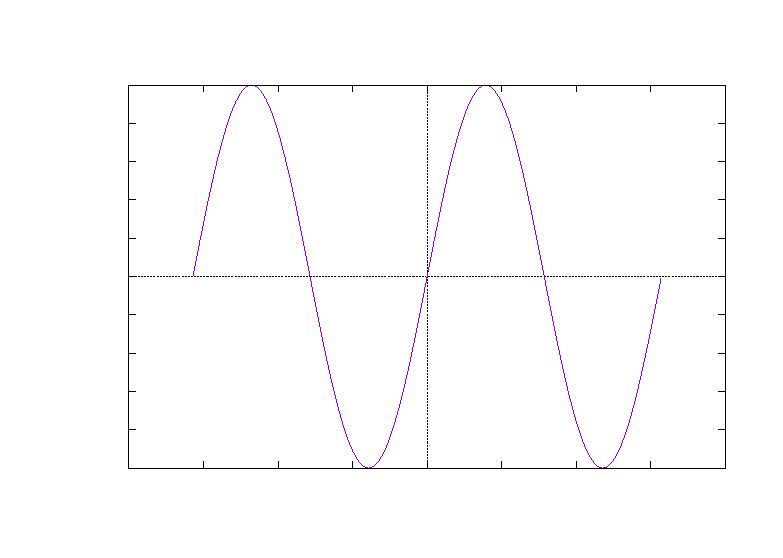
\includegraphics[width={360.00bp},height={252.00bp}]{figures/sinplot}}%
    \gplfronttext
  \end{picture}%
\endgroup

  \caption{\label{figure:sinplot}
    Values of $\sin(x)$ over $x$ in $[-2\pi, 2\pi)$.
  }
\end{figure}

% Use pylisting for nicer colors.
\begin{pylisting}{\texttt{plot.sh}}
#!/bin/bash

make clean && make sincos   # Rebuild the sincos executable.
./sincos > /tmp/sin.dat     # Place the data points into a file.

# This is the here-document that is sent to gnuplot.
gnuplot <<END
    set terminal pdf
    set output "sin.pdf"
    set title "sin(x)"
    set xlabel "x"
    set ylabel "y"
    set zeroaxis
    plot "/tmp/sin.dat" with lines title ""
END
\end{pylisting}

The first line, although it starts with the comment character \texttt{\#}, is
imperative. It acts as the \emph{interpreter directive}. When \texttt{plot.sh}
is executed, the first two bytes of the file, \texttt{\#!}, indicate that
\texttt{plot.sh} is a executable script and the program to use to interpret
the script is \texttt{/bin/bash}. To set the executable bit of
\texttt{plot.sh}, use \texttt{chmod}:

\begin{shlisting}{}
$ chmod +x plot.sh
\end{shlisting}

To run the script:

\begin{shlisting}{}
$ ./plot.sh
\end{shlisting}

The syntax for a here-document may look a little strange. An identifier is
required to delineate the start and end of the here-document. In the case of
\texttt{plot.sh}, the identifier \texttt{END} is used. Any identifier is fine as
long as the contents of the here-document don't also use the identifier. It
should be clear that \texttt{gnuplot} is the intended destination command for
this particular here-document, but here-documents in general can be sent to any
command.

\section{Useful Commands}

This section will cover some commands that you'll find useful for this
assignment and for the course in general. This is not meant to be an exhaustive
list. We will cover all the commands that were used to create Figures
\ref{figure:collatz-length}, \ref{figure:collatz-maxval}, and
\ref{figure:collatz-hist}, but you may end up using commands that aren't listed.

\begin{itemize}
  \item \texttt{head} --- Prints out the first 10 lines of a file by default.
    Can be instructed to print out a specific number of lines.
  \item \texttt{ls} --- Lists the contents of the current working directory.
  \item \texttt{sort} --- Prints the sorted contents of a file. The contents are
    sorted lexicographically by default, but can be specified to be sorted
    numerically if desired.
  \item \texttt{uniq} --- Filters out repeated lines in a file. Can be used to
    both filter out repeated lines and count the number of times a line was
    repeated.
  \item \texttt{wc} --- Prints out the word, line, and character count of a
    file.
\end{itemize}

We have provided a brief description for each command, but should you find
yourself wanting more information, refer to the command's \texttt{man} page. You
can do so using \texttt{man <command>}. A \texttt{man} page (short for manual
page) is software documentation for tools and programs found on \Unix{} systems.
To view a \texttt{man} page:

\begin{shlisting}{}
$ man <function, program, tool>
\end{shlisting}

These manual pages are typically divided into sections, depending on
their respective purposes. General commands are found in section 1,
system calls in section 2, and library functions, such as the
\texttt{printf()} function used in this assignment, are found in section
3. So, to view the \texttt{man} page for \texttt{printf()}:

\begin{shlisting}{}
$ man 3 printf
\end{shlisting}

You will want to get into the habit of checking \texttt{man} pages. They are
written by programmers for programmers and will be invaluable when you get to
writing \C{} code.

\section{Deliverables}

\epigraphwidth=0.4\textwidth
\epigraph{\emph{It is such a sweet temptation \\ It gives such grief relief \\
It is such a false sensation \\ How come that's so hard to believe?}}{---Ray
Wylie Hubbard, \emph{Loco Gringo's Lament}}

You will need to turn in the following source code and header files:

\begin{enumerate}
  \item Your program \emph{must} have the following source and header
    files:
  \begin{itemize}
    \item \texttt{universe.c} implements the \texttt{Universe} ADT.
    \item \texttt{universe.h} specifies the interface to the \texttt{Universe}
      ADT. This file is provided and \emph{may not} be modified.
    \item \texttt{life.c} contains \texttt{main()} and \emph{may}
      contain any other functions necessary to complete your implementation of
      the Game of Life.
  \end{itemize}
\end{enumerate}

You can have other source and header files, but \emph{do not try to be overly
clever}. You will also need to turn in the following:

\begin{enumerate}
  \item \texttt{Makefile}:
    \begin{itemize}
      \item \texttt{CC = clang} must be specified.
      \item \texttt{CFLAGS = -Wall -Wextra -Werror -Wpedantic} must be specified.
      \item \texttt{make} must build the \texttt{life} executable, as should
        \texttt{make all} and \texttt{make life}.
      \item \texttt{make clean} must remove all files that are compiler
        generated.
      \item \texttt{make format} should format all your source code,
        including the header files.
    \end{itemize}
  \item \texttt{README.md}: This must use proper Markdown syntax. It
    must describe how to use your program and \texttt{Makefile}. It
    should also list and explain any command-line options that your
    program accepts. Any false positives reported by \texttt{scan-build}
    should be documented and explained here as well. Note down any known
    bugs or errors in this file as well for the graders.
  \item \texttt{DESIGN.pdf}: This document \emph{must} be a proper
    PDF\@. This design document must describe your design and design
    process for your program with enough detail such that a sufficiently
    knowledgeable programmer would be able to replicate your
    implementation. \textcolor{red}{This does not mean copying your
    entire program in verbatim}. You should instead describe how your
    program works with supporting pseudocode.
  \item \texttt{WRITEUP.pdf}: This document \emph{must} be a proper
    PDF\@. This writeup document must include everything you learned from
    this assignment. Make sure to mention everything in detail while being as precise as possible. How well you explain all the lessons you have learned in this assignment will be really important here. 
\end{enumerate}

\section{Submission}

Refer back assignment 0 for the instructions on how to properly submit
your assignment through \texttt{git}. Remember: \emph{add},
\emph{commit}, and \emph{push}!

\textcolor{red}{Your assignment is turned in \emph{only} after you have
pushed and submitted the commit ID you want graded on Canvas. ``I
forgot to push'' and ``I forgot to submit my commit ID'' are not valid
excuses. It is \emph{highly} recommended to commit and push your changes
\emph{often}.}

\section{Supplemental Readings}

\epigraph{\emph{The more that you read, the more things you will know. The
more that you learn, the more places you'll go.}}{---Dr.\ Seuss}

\begin{itemize}
  \item \textit{The C Programming Language} by Kernighan \& Ritchie
  \begin{itemize}
    \item Chapter 7
    \item Appendix B
  \end{itemize}
  \item \textit{Introduction to Algorithms} by T.\ Cormen, C.\
    Leiserson, R.\ Rivest, \& C.\ Stein
    \begin{itemize}
      \item Chapter 31 \S 31.2, \S 31.3, \S 31.6, \S 31.7, \S 31.8
    \end{itemize}
\end{itemize}


\vfill
\begin{center}
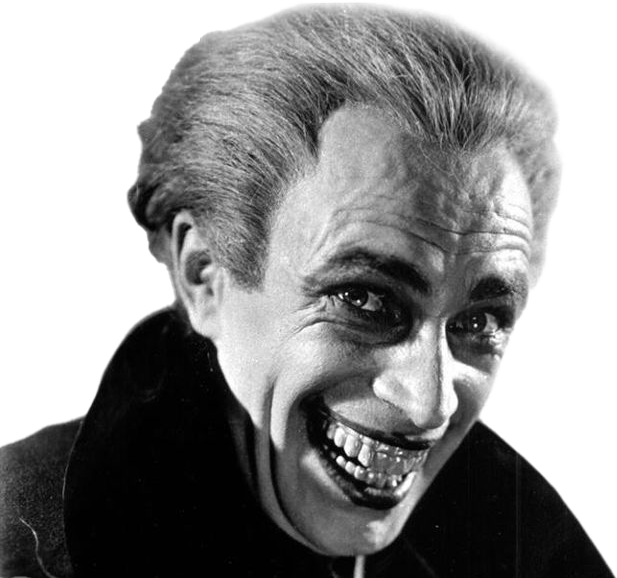
\includegraphics[width=0.3\textwidth]{images/cv.png} \\
\emph{Honi soit l'homme qui rit.}
\end{center}
\end{document}
